\documentclass[tikz,border=2pt]{standalone}
\usepackage{tgheros}
\usetikzlibrary{arrows.meta}

\begin{document}
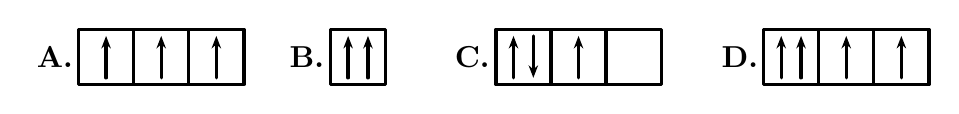
\begin{tikzpicture}[line cap=round, line join=round]
  \def\s{0.7} % kích thước mỗi ô vuông 0.7cm x 0.7cm
  \tikzset{
    box/.style={line width=1.2pt, draw=black},
    spin_up/.style={line width=1.2pt, -{Stealth[length=4.5pt, width=3.4pt]}, draw=black},
    spin_down/.style={line width=1.2pt, -{Stealth[length=4.5pt, width=3.4pt]}, draw=black}
  }


  \node[font=\bfseries\fontsize{11pt}{13pt}\selectfont] at (-0.3, 0.35) {A.};
  \draw[box] (0, 0) rectangle (\s, \s);
  \draw[box] (\s, 0) rectangle (2*\s, \s);
  \draw[box] (2*\s, 0) rectangle (3*\s, \s);
  \draw[spin_up] (0.5*\s, 0.12*\s) -- (0.5*\s, 0.88*\s);
  \draw[spin_up] (1.5*\s, 0.12*\s) -- (1.5*\s, 0.88*\s);
  \draw[spin_up] (2.5*\s, 0.12*\s) -- (2.5*\s, 0.88*\s);

  \begin{scope}[xshift=3.2cm]
    \node[font=\bfseries\fontsize{11pt}{13pt}\selectfont] at (-0.3, 0.35) {B.};
    \draw[box] (0, 0) rectangle (\s, \s);
    \draw[spin_up] (0.32*\s, 0.12*\s) -- (0.32*\s, 0.88*\s);
    \draw[spin_up] (0.68*\s, 0.12*\s) -- (0.68*\s, 0.88*\s);
  \end{scope}

  \begin{scope}[xshift=5.3cm]
    \node[font=\bfseries\fontsize{11pt}{13pt}\selectfont] at (-0.3, 0.35) {C.};
    \draw[box] (0, 0) rectangle (\s, \s);
    \draw[box] (\s, 0) rectangle (2*\s, \s);
    \draw[box] (2*\s, 0) rectangle (3*\s, \s);
    \draw[spin_up] (0.32*\s, 0.12*\s) -- (0.32*\s, 0.88*\s);
    \draw[spin_down] (0.68*\s, 0.88*\s) -- (0.68*\s, 0.12*\s);
    \draw[spin_up] (1.5*\s, 0.12*\s) -- (1.5*\s, 0.88*\s);
  \end{scope}

  \begin{scope}[xshift=8.7cm]
    \node[font=\bfseries\fontsize{11pt}{13pt}\selectfont] at (-0.3, 0.35) {D.};
    \draw[box] (0, 0) rectangle (\s, \s);
    \draw[box] (\s, 0) rectangle (2*\s, \s);
    \draw[box] (2*\s, 0) rectangle (3*\s, \s);
    \draw[spin_up] (0.32*\s, 0.12*\s) -- (0.32*\s, 0.88*\s);
    \draw[spin_up] (0.68*\s, 0.12*\s) -- (0.68*\s, 0.88*\s);
    \draw[spin_up] (1.5*\s, 0.12*\s) -- (1.5*\s, 0.88*\s);
    \draw[spin_up] (2.5*\s, 0.12*\s) -- (2.5*\s, 0.88*\s);
  \end{scope}


\end{tikzpicture}
\end{document}
